%++++++++++++++++++++++++++++++++++++++++
% Don't modify this section unless you know what you're doing!
%\documentclass[letterpaper,12pt]{article}
\documentclass[a4paper]{article}
\usepackage{tabularx} % extra features for tabular environment
\usepackage{amsmath}  % improve math presentation
\usepackage{graphicx} % takes care of graphic including machinery
%\usepackage[margin=1in,letterpaper]{geometry} % decreases margins
\usepackage{cite} % takes care of citations
%\usepackage[final]{hyperref} % adds hyper links inside the generated pdf file
%\hypersetup{
%	colorlinks=true,       % false: boxed links; true: colored links
%	linkcolor=blue,        % color of internal links
%	citecolor=blue,        % color of links to bibliography
%	filecolor=magenta,     % color of file links
%	urlcolor=blue
%}
%++++++++++++++++++++++++++++++++++++++++
\usepackage{indentfirst}
\usepackage{tensor}
\usepackage{amssymb}
\allowdisplaybreaks
\usepackage{bm}
\newcommand{\at}[2][]{#1|_{#2}}
\newcommand\numberthis{\addtocounter{equation}{1}\tag{\theequation}}
\newcommand\norm[1]{\left\lVert#1\right\rVert}

% Python code, taken from:
% https://www.quora.com/What-is-the-optimal-way-to-include-Python-code-in-a-LaTeX-document
\usepackage{color}
\usepackage{listings}
\usepackage{setspace}
\definecolor{Code}{rgb}{0,0,0}
\definecolor{Decorators}{rgb}{0.5,0.5,0.5}
\definecolor{Numbers}{rgb}{0.5,0,0}
\definecolor{MatchingBrackets}{rgb}{0.25,0.5,0.5}
\definecolor{Keywords}{rgb}{0,0,1}
\definecolor{self}{rgb}{0,0,0}
\definecolor{Strings}{rgb}{0,0.63,0}
\definecolor{Comments}{rgb}{0,0.63,1}
\definecolor{Backquotes}{rgb}{0,0,0}
\definecolor{Classname}{rgb}{0,0,0}
\definecolor{FunctionName}{rgb}{0,0,0}
\definecolor{Operators}{rgb}{0,0,0}
\definecolor{Background}{rgb}{0.98,0.98,0.98}
\lstset{
    breaklines=true,
    postbreak=\mbox{\textcolor{red}{$\hookrightarrow$}\space}
}
\lstdefinelanguage{Python}{
numbers=left,
numberstyle=\footnotesize,
numbersep=1em,
xleftmargin=1em,
framextopmargin=2em,
framexbottommargin=2em,
showspaces=false,
showtabs=false,
showstringspaces=false,
frame=l,
tabsize=4,
% Basic
basicstyle=\ttfamily\small\setstretch{1},
backgroundcolor=\color{Background},
% Comments
commentstyle=\color{Comments}\slshape,
% Strings
stringstyle=\color{Strings},
morecomment=[s][\color{Strings}]{"""}{"""},
morecomment=[s][\color{Strings}]{'''}{'''},
% keywords
morekeywords={import,from,class,def,for,while,if,is,in,elif,else,not,and,or,print,break,continue,return,True,False,None,access,as,,del,except,exec,finally,global,import,lambda,pass,print,raise,try,assert},
keywordstyle={\color{Keywords}\bfseries},
% additional keywords
morekeywords={[2]@invariant,pylab,numpy,np,scipy},
keywordstyle={[2]\color{Decorators}\slshape},
emph={self},
emphstyle={\color{self}\slshape},
%
}
\linespread{1.3}
% Python code [end].

\usepackage{caption}
\captionsetup[lstlisting]{font={small}}
\renewcommand{\lstlistingname}{Algorithm}

% Fontsize of figure smaller than normalsize:
\captionsetup[figure]{font=small}
\captionsetup[table]{font=small}

\usepackage{breqn}

\begin{document}

\title{Atari Breakout with\\$\text{LTL}_f\text{/LDL}_f$ Goals}
%\author{Ivan Bergonzani, Michele Cipriano, Armando Nania}
%\date{\today}
%\maketitle


\makeatletter
\let\thetitle\@title
\let\theauthor\@author
\let\thedate\@date
\makeatother

\begin{titlepage}
	\centering
    \vspace*{0.5 cm}
    
\includegraphics[scale = 0.75]{images/SapienzaLogo}\\[1.0 cm]	% University Logo

    \vspace*{-0.3cm}
    \textsc{\large Department of Computer, Control and\\Management Engineering}\\[2.0 cm]	% Department Name
    \vspace*{1.2cm}

    { \fontsize{20.74pt}{18.5pt}\selectfont\bfseries \thetitle \par } % title

    \vspace*{0.1cm}
    \textsc{\Large Elective in Artificial Intelligence:\\Reasoning Robots}\\[0.5 cm] % course name

    \vspace*{2.8cm}
	\begin{minipage}{0.4\textwidth}
		\begin{flushleft} \large
			\emph{Professor:}\\
			Giuseppe De Giacomo\\
            %Computer Science Department\\
		\end{flushleft}
	\end{minipage}~
	\begin{minipage}{0.4\textwidth}
		\begin{flushright} \large
			\emph{Students:} \\
            Ivan Bergonzani \\
			Michele Cipriano\\
            Armando Nania
            %Semester\\
		\end{flushright}

	\end{minipage}\\[2 cm]

    \vspace{0.2cm}
    \rule{\linewidth}{0.2 mm} \\[0.3 cm]
    \vspace*{-0.3cm}
    Academic Year 2017/2018
\end{titlepage}

\tableofcontents
\newpage


%\begin{abstract}
%In this experiment we studied a very important physical effect by measuring the
%dependence of a quantity $V$ of the quantity $X$ for two different sample
%temperatures.  Our experimental measurements confirmed the quadratic dependence
%$V = kX^2$ predicted by Someone's first law. The value of the %mystery parameter
%$k = 15.4\pm 0.5$~s was extracted from the fit. This value is
%not consistent with the theoretically predicted $k_{theory}=17.34$~s. We attribute this
%discrepancy to low efficiency of our $V$-detector.
%\end{abstract}

\section{Introduction}
Introduction to the whole project, structure of the report and summary of
the work.

\clearpage

\section{Reinforcement Learning}
Reinforcement learning \cite{Suttonrl18} is an area of machine learning
which aims at studying how to develop agents that can interact with
their environment maximing a cumulative reward. The environment can be
formally defined as a Markov Decision Process (MDP), which is a tuple
$\langle S, A, \delta, R \rangle$ where $S$ is a finite set of states that can represent
the environment, $A$ is a finite set of actions that can be perform by
an agent in the environment, $\delta$ is a probability function modeling
the transition from a state to another when performing a certain action and
$R$ is a reward function which models the reward received by the environment
when performing a certain action which makes the agent move from a state
to another.

An interesting property of the MDP is that it satisfies the Markov property,
hence, the future states that will be reached by the agent do not depend
on the past interaction of the environment, but just on the current state.
This makes it possbile to define the transition and the reward function
depending only on the current state (and of course the action and the future
state of interest).

This section considers two common reinforcement learning algorithm,
namely Q-Learning and SARSA, which have been used in our experiments
in order to train an agent interacting with an Atari Breakout environment
(section \ref{subsec:experiments}).

\subsection{Q-Learning}
Q-Learning is a temporal difference (TD) algorithm that directly approximates
the optimal action-value
function. This method guarantees to find an optimal behaviour under the
assumption that the all state-action pairs are updated infinitely many times. It is
defined \cite{Suttonrl18} by the following equation:
\begin{equation}
    \label{eq:qlearning-update-function}
    Q(S_t, A_t) \leftarrow Q(S_t, A_t) + \alpha \Big[ R_{t+1} +
        \gamma \max_{a} Q(S_{t+1}, a) - Q(S_t, A_t) \Big]
\end{equation}

Let's briefly discuss the implementation used in our project by studying
the Python implementation (Algorithm \ref{lst:qlearning-py}). The algorithm
is defined by the class \texttt{QLearning} that extends the abstract class
\texttt{TDBrain}. The constructor of the class (lines 2-4) simply calls its
parent constructor that will initialize the parameters of the object, hence,
the observation space and the action space (\texttt{gym} objects), the strategy
used by the policy function, which is $\varepsilon$-greedy by default and the
hyperparameters $\gamma$, $\alpha$ and $\lambda$ of the upper class.
The abstract method inherited from \texttt{TDBrain} is \texttt{update\_Q},
which should be implemented in order to define how to update the action-state
table. The method (lines 6-21) simply follows Eq.
\ref{eq:qlearning-update-function}. TODO: eligibility.
\lstinputlisting[caption=Q-Learning algorithm Python implementation.,
    label={lst:qlearning-py},
    language=Python]{implementation/TDBrain-QLearning.py}

\subsection{SARSA}
A similar TD algorithm is the SARSA algorithm, which name
comes from the fact that at each timestep a quintuple $\langle S_t, A_t,
R_{t+1}, S_{t+1}, A_{t+1} \rangle$ is considered. As before, SARSA converges
to an optimal action-value function under the assumption that all state-action
pairs are updated infinitely many times. It is defined
\cite{Suttonrl18} by the following equation:
\begin{equation}
    \label{eq:sarsa-update-equation}
    Q(S_t, A_t) \leftarrow Q(S_t, A_t) + \alpha \Big[ R_{t+1} +
        \gamma Q(S_{t+1}, A_{t+1}) - Q(S_t, A_t) \Big]
\end{equation}

Let's briefly discuss the implementation used in our project by studying the
implementation (Algorithm \ref{lst:sarsa-py}), as done before with the
Q-Learning algorithm. Again, the algorithm is defined by the class
\texttt{Sarsa} that extends the abstract class \texttt{TDBrain}. The constructor
of the class (lines 2-4) calls its parent constructor initializing the
parameters of the upper class exactly in the same way as the class
\texttt{QLearning}. The class implements the inherited method
\texttt{update\_Q} by following Eq. \ref{eq:sarsa-update-equation} (lines
6-17). TODO: eligibility.
\lstinputlisting[caption=SARSA algorithm Python implementation.,
    label={lst:sarsa-py},
    language=Python]{implementation/TDBrain-Sarsa.py}

\clearpage

\section{$\text{LTL}_f\text{/LDL}_f$ Non-Markovian Rewards}
\label{section:nonmarkovianrewards}
Recently, non-Markovian reward decision processes (NMRDPs)
have attracted interest in the scientific community because of the possibility
of specifying them as MDPs with $\text{LTL}_f\text{/LDL}_f$ non-Markovian
rewards \cite{DBLP:journals/corr/abs-1807-06333}. In particular, it is possible
to model the problem with two separate representations of the world, one for
the agent (low-level) and one for the goal (expressed in terms of high-level
fluents).

This section presents the approach used in
\cite{DBLP:journals/corr/abs-1807-06333}, where an efficient method has been
developed in order to work with NMRDPs. The theory behind the main idea is
quickly described and an example on a theoretical Breakout environment is
discussed in order to be used in the following sections easily.

\subsection{Theoretical Background}
Before describing the problem, let's give a formal definition of NMRDP.
A non-Markovian reward decision process is a tuple $M = \langle S, A, \delta,
\bar{R} \rangle$, with $S$ finite set of states that can represent the
environment, $A$ is a finite set of actions that can be performed by an agent
in the environment, $\delta$ is a probability function modeling
the transition from a state to another when performing a certain action and
$\bar{R}: (S \times A)^* \rightarrow \mathbb{R}$ is a function from
finite state-action sequences (traces) to real-values that represents the
reward given by the environment when performing a certain state-action
sequence. Specifying a non-Markovian reward function explicitely is
difficult even when considering a finite number of traces. Luckily, the
$\text{LTL}_f\text{/LDL}_f$ formalism allows to specify $\bar{R}$
implicitely using a set of pairs $\{ (\phi_i, r_i) \}_{i=1}^m$ with
$\phi_i$ boolean
proposition over the components of the state vector and $r_i$ such that,
given a current trace $\pi = \langle s_, a_1, \dots, s_{n-1}, a_n \rangle$,
the agent receives at $s_n$ a reward $r_i$ if $\phi_i$ is satisfied by $\pi$,
hence:
\begin{equation}
    \bar{R}(\pi) =
        \begin{cases}
            r_i & \text{if } \pi \vDash \phi_i \\
            0 & \text{otherwise}
        \end{cases}
\end{equation}

Since the NMRDP rewards are based on traces, instead of state-action pairs,
typical learning algorithms like Q-learning or SARSA cannot be used.
Nevertheless, it has been shown \cite{DBLP:journals/corr/abs-1807-06333} that
for any NMRDP $M = \langle S, A, \delta, \{ (\phi_i, r_i) \}_{i=1}^m \rangle$
there exists an MDP $M' = \langle S', A', \delta' R' \rangle$ that is equivalent
to $M$. The idea behind the proof consists in starting from an initial
decision process $M_{ag}^{goal} = \langle S, A, R, \mathcal{L},
\delta_{ag}^g, \{ (\phi_i, r_i) \}_{i=1}^m \rangle$ with
$\text{LTL}_f\text{/LDL}_f$ goals (with $\mathcal{L}$ set of of configuration
of the high-level features needed for expressing $\phi_i$),
transform it into a NMRDP in order to
further transform it into a MDP where it is possible to execute learning
algorithms such as Q-learning. All the details are out of the scope of the
project and are discussed in \cite{DBLP:journals/corr/abs-1807-06333}. The
set of states $S$ is used to express low-level features of the agent.

The new MDP is extended by using automata needed to track the satisfiability
of a $\text{LTL}_f\text{/LDL}_f$ formulas, as explained in
\cite{DBLP:conf/aaai/2018}. Each formula is, hence, associated with an
automaton that accepts exactly the traces satisfying the formula itself.

Once the MDP has been determined it is possible to train a model that will
be able to manage non-Markovian rewards as well. Fig.
\ref{fig:rl-temporalgoals-pipeline} shows a pipeline of the
agent interacting with the world. In particular, a robot feature extractor
will analyze the state of the world $w$ in order to pass a representation $s$ to the
agent, a goal feature extractor will extract higher-level features $l$ of the world
that can be used to determine if a temporal goal has been achieved or not. In
positive case a reward $r$ is given to the agent. The evaluation $q$ of the formula
that specifies the temporal goals is given to the learning agent as well, in
order to construct an extended state of the MDP as specified by the theory above.
Each time the learning agent performs an action $a$, the environment changes
and it gives to the agent a reward $R$.
\begin{figure}
    \centering
    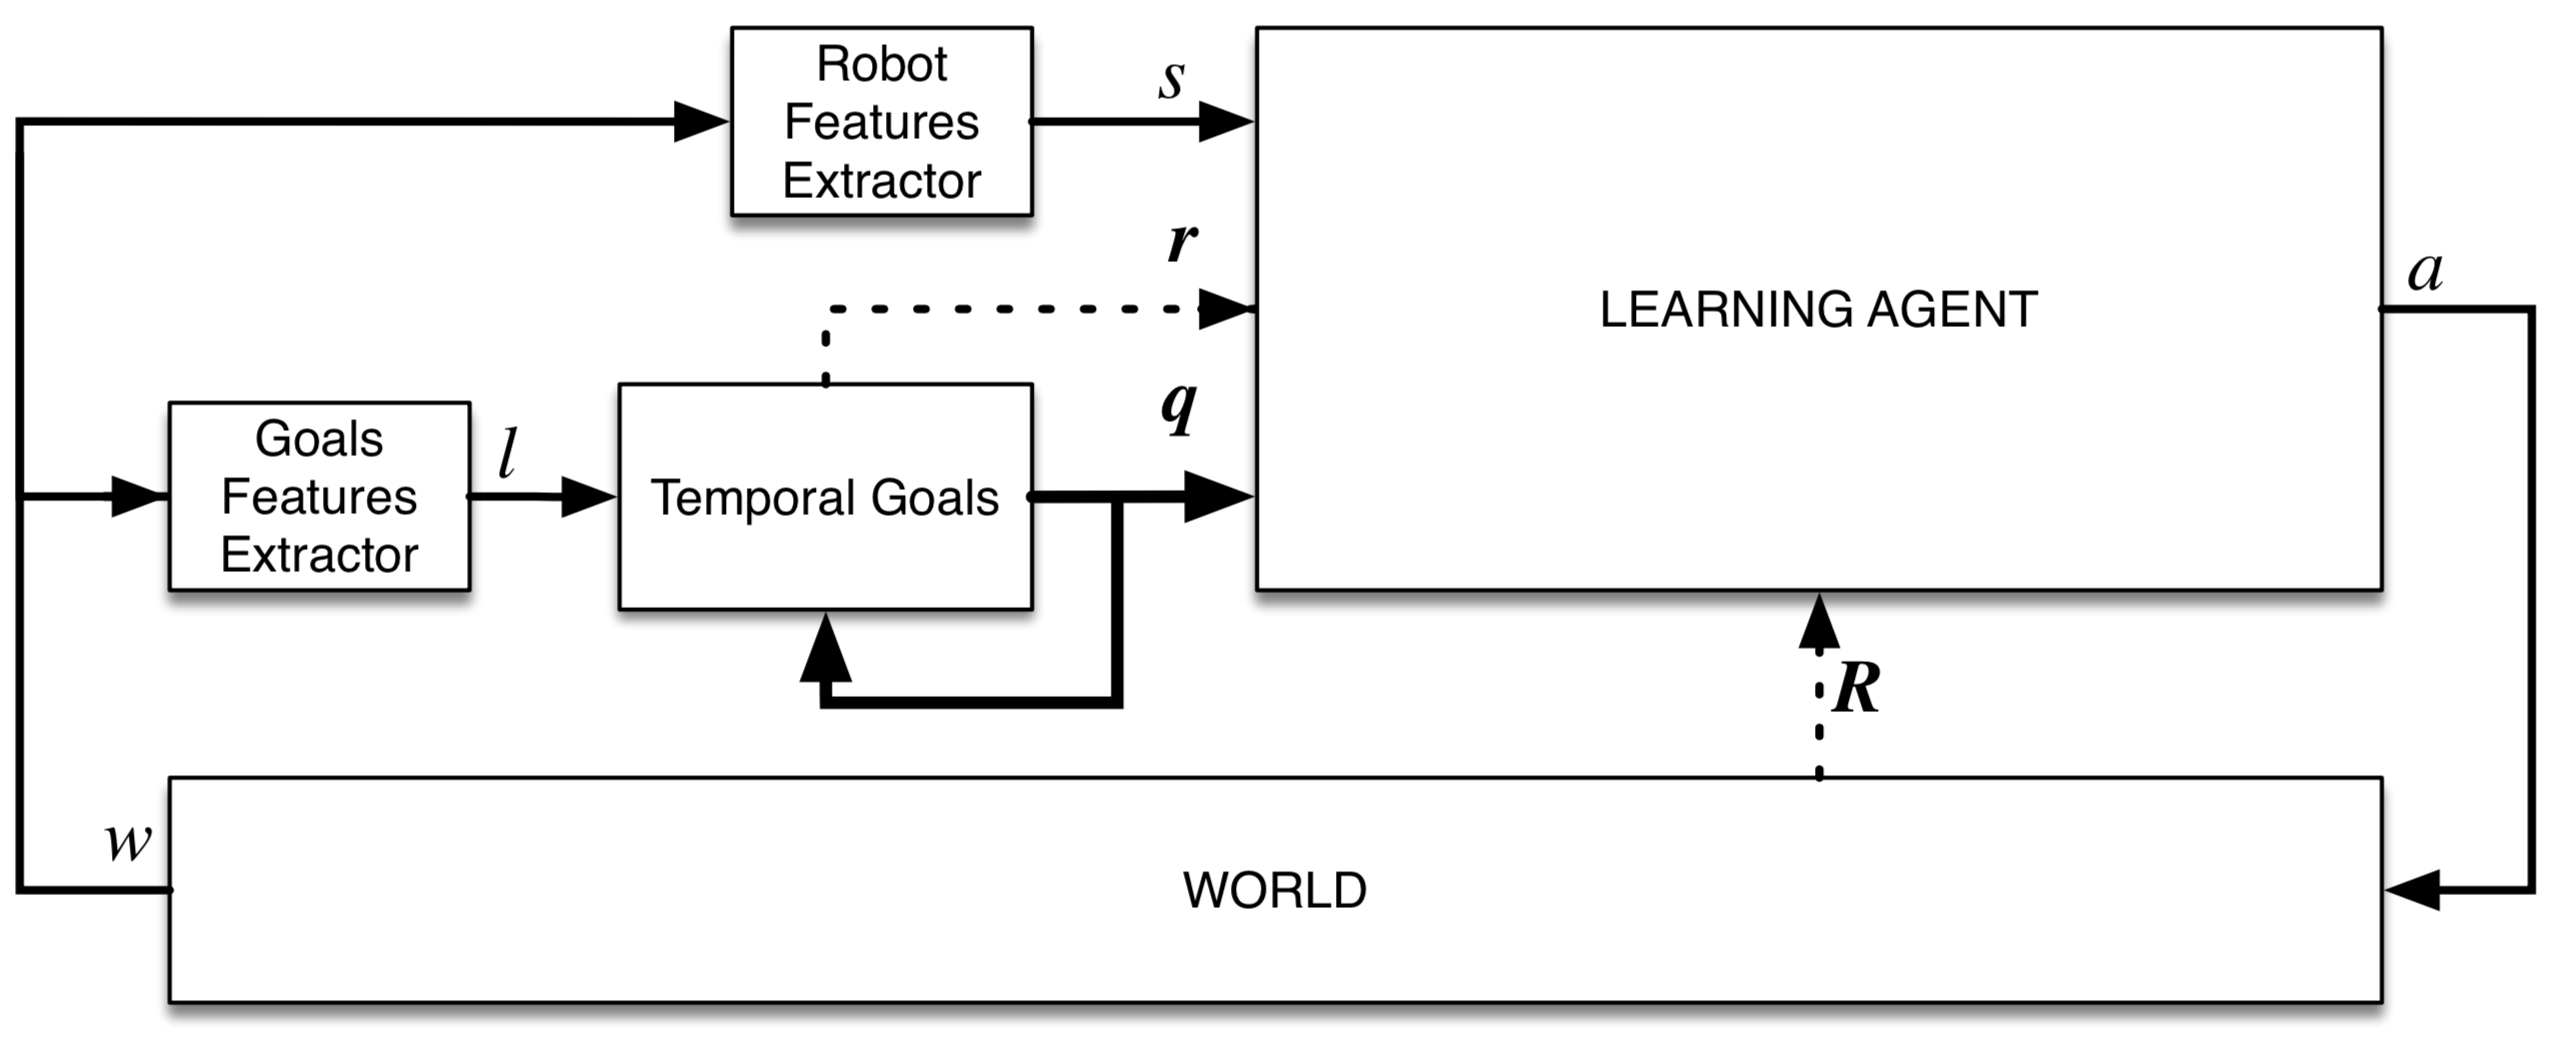
\includegraphics[width=0.85\textwidth]{images/rl-temporalgoals-pipeline.png}
    \caption{Pipeline describing how the agent is interacting with the
        world and how the robot features extractor and the goal features
        extractor are used in order to handle non-Markovian rewards.}
    \label{fig:rl-temporalgoals-pipeline}
\end{figure}

\subsection{Examples}
A typical example is breaking the bricks of a theoretical Breakout game in a
certain order. Let's consider a 3$\times$3 Breakout. A good idea is to use
$\text{LTL}_f\text{/LDL}_f$ goals to help the agent break to bricks from top
to bottom in order to make it create a hole on the left (or the right) and let
the ball do all the job without making any movements when it reaches the top
part of the environment. The idea is, hence, to help the agent learn
the most effective strategy, which should also decrease the training time.
Let's consider a formula that checks weather a row has been broken or not:
\begin{align}
\begin{split}
    \langle&(\neg\varphi_0 \land \neg\varphi_1 \land \neg\varphi_2)^*;
        (\varphi_0 \land \neg\varphi_1 \land \neg\varphi_2);
        (\varphi_0 \land \neg\varphi_1 \land \neg\varphi_2)^*;\\
        &(\varphi_0 \land \varphi_1 \land \neg\varphi_2);
        (\varphi_0 \land \varphi_1 \land \neg\varphi_2)*;
        (\varphi_0 \land \varphi_1 \land \varphi_2)\rangle tt
\end{split}
\end{align}

\noindent which, given $\varphi_0$ first row from the top broken,
$\varphi_1$ second row from the top broken and $\varphi_2$ third row from the
top broken, can be interpreted as:
\begin{itemize}
    \item $(\neg\varphi_0 \land \neg\varphi_1 \land \neg\varphi_2)^*$:
        initially, and for an indefinite amout of time, none of the rows have
        been broken;
    \item $(\varphi_0 \land \neg\varphi_1 \land \neg\varphi_2)$: then,
        the first row from the top has been broken but the remaining two
        are intact;
    \item $(\varphi_0 \land \neg\varphi_1 \land \neg\varphi_2)^*$: then,
        for an indefinite amount of time, the first row remains broken
        and the remaining two remain intact;
    \item $(\varphi_0 \land \varphi_1 \land \neg\varphi_2)$: then,
        the first two rows from the top have been broken and the remaining
        one at the bottom is intact;
    \item $(\varphi_0 \land \varphi_1 \land \neg\varphi_2)*$: then,
        for an indefinite amount of time, the first two rows from the top
        remain broken and the last one remain instact;
    \item $(\varphi_0 \land \varphi_1 \land \varphi_2)$: in the end,
        all the rows have been broken, hence, all the bricks have been broken.
\end{itemize}

In general, the formula $\langle\rho\rangle\phi$ states that, from the current step in
the trace, there exists an execution satifying $\rho$ such that in its last
step $\phi$ is satisfied. In the example above, at the end of the execution all
the rows have been broken.

\clearpage

\section{OpenAI Gym}
\label{sec:openaigym}
OpenAI \texttt{gym} \cite{1606.01540} is a toolkit for developing and comparing
reinforcement learning algorithms, without making assumptions about the
structure of the agent interacting with the environment, in order to
keep development flexible to updates on both sides.

\subsection{Framework}
The framework of \texttt{gym} allows to interact easily
with an environment, giving the developers to tools they need to perform
actions and to observe the state of the environment itself. In this way it is
possible to focus more on the development of the agent without spending
time on the structure of the world.

\texttt{gym} makes it possible to interact with multiple kinds of environments.
Among these, the authors of the framework developed the support for
Arcade Learning Environment \cite{bellemare13arcade}, which includes all the
classing Atari games, including Breakout, which has been used in this project.

\subsection{Examples}
Let's consider a simple example to understand how \texttt{gym} works and
how the framework can be used to interact with an environment.
The description will follow Algorithm \ref{lst:gym-breakout-example-py}.

\lstinputlisting[caption={Example of a random interaction with the \texttt{gym}
    environment \texttt{BreakoutNoFrameskip-v4}, used also in our experiments
    of subsection \ref{subsec:experiments}.},
    label={lst:gym-breakout-example-py},
    language=Python]{implementation/gym-breakout-example.py}

Initially (line 1) the framework is imported. Then (line 3-4) an environment
is created specifying its name and initializing it. The program makes a
random agent interact randomly with the environment for 1000 episodes (lines
6-11) before closing the environment. Line 7 renders the current
observation of the environment on screen, line 8-9 performs a random action
between those available in this Brekout version, note that the method
\texttt{step} return an \texttt{observation} (shown in Fig.
\ref{fig:gym-breakout-image-example}), which is an array of pixels
that represent the current state of the environment, a \texttt{reward},
which is a value return by the game after performing the specified action
\texttt{action}, a boolean value \texttt{done}, which is \texttt{True} is
the game is over, \texttt{False} otherwise, and \texttt{info} which contains
extra information about the game. Lines 10-11 handles the case when the game
is over, resetting the environment.

\begin{figure}
    \centering
    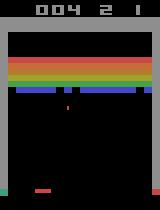
\includegraphics[width=0.3\textwidth]{images/gym-breakout-image-example.jpg}
    \caption{Observation of a frame of the environment
        \texttt{BreakoutNoFrameskip-v4}.}
    \label{fig:gym-breakout-image-example}
\end{figure}

\clearpage

\section{Atari Breakout}
This section contains the main part of the project, describing in detail our
starting point, how the program has been developed, the results achieved and the
comparison with the original implementation, which uses a non-Atari version
of the game Breakout \cite{DBLP:journals/corr/abs-1807-06333} with the same
number of bricks used in the Atari implementation of \texttt{gym},
already introduced in section \ref{sec:openaigym}.

Initially, the non-Atari version of Breakout (built on PyGame) is introduced,
its implementation is discussed and the results on the training with a brick
matrix of dimension 6$\times$18 are presented. Then the \texttt{gym}
environment \texttt{BreakoutNoFrameskip-v4} is presented and compared with the
PyGame breakout. A detailed description of the implementation of the project
is described, discussing in detail how the features have been extracted from
the environment (both the robot and the goal features), how temporal goals
have been used to evaluate the state of the bricks and how everything is
connected together in order to make it work with \texttt{gym}. In the end,
the main experiments performed on \texttt{BreakoutNoFrameskip-v4} are
presented.

\subsection{PyGame Breakout}
As introduced above, in \cite{DBLP:journals/corr/abs-1807-06333} a PyGame
version of the Breakout game has been used in order to test the algorithms
introduced in the paper. The implementation of this Breakout easily allows
to determine the state of the environment, saving the status of the bricks
(either in the scene or broken), the position of the ball, the direction of
the ball and the position of the paddle. This makes it possible to reduce
a lot the computational time of the implementation of the agent since the
data it receives are already preprocessed in order to have a complete
overview of the environment, allowing to focus on higher-level reasoning
tasks.

Originally, the paper focused on a Breakout environment with a brick matrix
of dimension 4$\times$5. Since the Atari version of Breakout is dealing with
a brick matrix of dimension 6$\times$18, a new test has been performed to
make the two environments comparable, in order to better understand the
potentiality of $\text{LTL}_f\text{/LDL}_f$, the use of non-Markovian rewards
and how to approach complex \texttt{gym} environments in the future.

The method managed to correctly break all the bricks in around one hour of
training. TODO: add three figures with initial state, middle, final.
TODO: add plot of rewards (shall this go to Experiments subsec?).

\subsection{Arcade Learning Environment}
This works aims at comparing the \texttt{gym} environment
\texttt{BreakoutNoFrameskip-v4}, already introduced in section
\label{sec:openaigym} with the non-Atari Breakout used in
\cite{DBLP:journals/corr/abs-1807-06333}. In last years, the reinforcement
learning community has grown a lot thanks to the introduction of \texttt{gym}
and deep reinforcement learning algorithms \cite{mnih2015humanlevel} that
managed to easily solve complex games that are considered difficult also
for humans, often achieving better results than expert human gamers. More
and more algorithms are introduced every year, exploiting GPU resources
and managing to solve harder games like Montezuma Revenge \cite{uber-goexplore}.
The popularity of deep reinforcement learning begun with the introduction of
Arcade Learning Environment (ALE) that includes most
famous arcade Atari games \cite{bellemare13arcade}.

The main characteristics of \texttt{gym} (or ALE) environments is that the
world can be observed only from the pixels of the screen, putting the
algorithms at the same level of the human, that can only observe the display
while playing. This makes the game a lot more complex since a more abstract
reasoning strategy is needed in order to solve the game. This hypothesis should
make \texttt{gym} games a lot harder than the non-Atari version of Breakout
that has been used to test algorithms that work with non-Markovian rewards.

\subsubsection{Atari Wrappers}
Before introducing the main part of the implementation it is important to
discuss the use of Atari wrappers, introduced with the OpenAI baselines
\cite{openai-baselines}, that simplify the interaction with the environment,
lightening the code and managing important aspects of the game.
The wrappers used in the project, as it is possible to notice from Algorithm
\ref{lst:run-atariwrappers-py}, are the following:
\begin{itemize}
    \item \texttt{EpisodicLifeEnv}: make an ``end of life'' be the end
        of the episode resetting the environment only on the true
        game over, this helps in value estimation;
    \item \texttt{FireResetEnv}: use ``Fire'' as starting action in order
        to launch the ball;
    \item \texttt{MaxAndSkipEnv}: returns only the skip-th frame, this
        reduces the amount of frame the agent has to deal with.
\end{itemize}

Note that line 1 defines the \texttt{gym} environment used in the project,
namely \texttt{BreakoutNoFrameskip-v4}. All the wrappers extend the class
\texttt{gym.Wrapper}.

\lstinputlisting[caption={Initialization of the Atari Breakout environment
    and the use of Atari wrappers from OpenAI.},
    label={lst:run-atariwrappers-py},
    language=Python]{implementation/breakoutfull-run-atariwrappers.py}

\subsection{Implementation}
Following the pipeline introduced in \cite{DBLP:journals/corr/abs-1807-06333}
and described in Fig. \ref{fig:rl-temporalgoals-pipeline}, the robot features
extractor, the goal features extractor and the temporal goals are described.
In particular, their implementation makes use of OpenCV \cite{opencv-library}
in order to deal
with images easily and a Python implementation of FLLOAT \cite{python-flloat}
to deal with $\text{LTL}_f\text{/LDL}_f$ formulas. Note that the abstract
class \texttt{TemporalEvaluator} in Algorithm \ref{lst:temporal-goals-py}
makes use of the libraries Pythomata \cite{pythomata} and RLTG \cite{rltg} to
build automata from the desired $\text{LTL}_f\text{/LDL}_f$ formulas in order
to make it possible to receive non-Markovian rewards.

\subsubsection{Robot Features Extractor}
The implementation of the robot features extractor is shown in Algorithm
\ref{lst:robot-features-extractor-py}. The class extends the abstract class
\texttt{BreakoutRobotFeatureExtractor}, which has been developed just to
keep a consistent structure among other implementation of other robot features
extractors. The class implements two methods: the constructor
\texttt{__init__}, which takes as input a \texttt{gym} object defining the space
of the observation, and the method \texttt{_extract}, which takes as input
the observation \texttt{input} coming from the environment and a dictionary
\texttt{kwargs} containing other optional parameters.

The constructor \texttt{__init__} defines the robot features space (lines 4-7)
with two \texttt{gym.spaces.Discrete} objects defined with values 287 and
157, respectively the maximum possible values (extreme excluded) that the
position of the ball can have with respect to the paddle and the height of the
ball. Then, internal representation of the position of the ball and of the
paddle are initialized (lines 9-12). The boolean \texttt{self.still_image}
is used to avoid repetitions of the same observation in the method
\texttt{_extract} since the same observation is considered twice. In the end,
the superconstructor is called (line 14) in order to finalize the
construction of the object.

The method \texttt{\_extract} checks weather the image has been already seen
or not (lines 17-19) has explained above. Then, the position of the paddle
is extracted from the observation (an image) on lines 20-35. Initially,
only the bottom part of the image is extracted from the observation (line 21),
it is then converted to a gray-scale image (line 22) so that it is possible
to apply a threshold function in order to make the paddle white and the
rest of the image black (line 23). In this way it is possible to find contours
of the objects contained in that part of the image (there should be only
one actually since only the bottom part is considered) and extract the centroid
of the paddle, in this way the variable
\texttt{paddleX} is updated. Similarly, the position of the ball is extracted
(lines 37-69) from the upper part of the image. Here, it is important to
actually check that the centroid is part of the ball since there could be
objects that are part of the bricks. Fortunately the ball has a unique RGB color
$(200, 72, 72)$ which simplifies this step.

Finally, the internal representation of the object is updated (lines 71-73)
and a tuple containing data specified in the constructor is returned (line 75).
\lstinputlisting[caption=Robot feature extractor Python implementation.,
    label={lst:robot-features-extractor-py},
    language=Python]{implementation/breakoutfull-breakoutrobotfeatureextractor.py}

\subsubsection{Goal Features Extractor}
The implementation of the goal features extractor is shown in Algorithm
\ref{lst:goal-features-extractor-py}. The class extends the abstract class
\texttt{FeatureExtractor}, which has been developed just to
keep a consistent structure among other implementation of other goal features
extractors. The class implements two methods: the constructor
\texttt{__init__}, which takes as input a \texttt{gym} object defining the space
of the observation and the number of rows and columns composing the bricks
matrix, and the method \texttt{_extract}, which takes as input
the observation \texttt{input} coming from the environment and a dictionary
\texttt{kwargs} containing other optional parameters.

The constructor \texttt{__init__} saves the number of rows and columns
(lines 3-4) of the
bricks matrix used in its internal representation and defines the space used
by the method \texttt{_extract} to return objects (a simple representation
of the bricks matrix). In the end, the superconstructor is called (line 6)
in order to finalize the construction of the object.

The method \texttt{\_extract} simply return a numpy representation of the
bricks matrix seen from the observation, which is return by the environment
each time the agent takes an action. The algorithm cycles on the pixels
of the image representing the observation checking weather they are black
or not. In particular, it is possible to determine this by checking the two
pixels on the upper left and upper right part of the brick comparing their
color (lines 10-20) with the background (black). If both of them are black, then the brick
has already been destroyed, otherwise it is still present in the environment.
Note that it is necessary to check both pixels because one of the two could
be different due to the presence of the ball during the game. As mentioned
above, the method return a 6$\times$18 numpy matrix representing the status of
the bricks (each element will have value 0 if the brick has been destroyed,
1 otherwise).
\lstinputlisting[caption=Goal feature extractor Python implementation.,
    label={lst:goal-features-extractor-py},
    language=Python]{implementation/breakoutfull-breakoutgoalfeatureextractor.py}

\subsubsection{Temporal Goals}
The implementation of temporal goals is shown in Algorithm
\ref{lst:temporal-goals-py}. It is divided in three parts:
\begin{itemize}
    \item \texttt{get_breakout_lines_formula}: a function that determines the
        $\text{LTL}_f\text{/LDL}_f$ formula as a string, in order to be
        later parsed by the FLLOAT parser;
    \item \texttt{BreakoutCompleteLinesTemporalEvaluator}: a
        temporal evaluator class that handles rows and columns as lines;
    \item \texttt{BreakoutCompleteRowsTemporalEvaluator}: a temporal evaluator
        class that extends \texttt{BreakoutCompleteLinesTemporalEvaluator} and
        work on rows, this is the main class used in the project regarding
        temporal goals.
\end{itemize}

In particular, \texttt{get_breakout_lines_formula} (lines 1-15) generates a
$\text{LTL}_f\text{/LDL}_f$ formula as explained in Section
\ref{section:nonmarkovianrewards}, but extended to a general case of a Breakout
consisting of a bricks matrix of size $n \times m$.

\texttt{BreakoutCompleteLinesTemporalEvaluator} extends the RLTG abstract class
\texttt{TemporalEvaluator} which contains the abstract method
\texttt{fromFeaturesToPropositional}. Its constructor \texttt{__init__} (lines
20-38) parses the $\text{LTL}_f\text{/LDL}_f$ specified by the function
\texttt{get_breakout_lines_formula} (lines 22-30) in order to pass it to
the superconstructor (lines 33-38) that will manage the construction of the
automata using Pythomata and RLTG libraries. The method
\texttt{fromFeaturesToPropositional}, inherited from \texttt{TemporalEvaluator},
maps the bricks matrix to a propositional formula in order to update the
automata while training the agent.

\texttt{BreakoutCompleteRowsTemporalEvaluator} has the same structure of the
previous class with the exception of the boolean \texttt{self.bottom_up} that
specifies weather breaking the rows from top to bottom or viceversa.
For all the experiments of the project this variable has been set to
\texttt{False} in order to incite the agent to find a strategy that makes the
ball go to the upper part of the environment in order to break the bricks
without making any effort.
\lstinputlisting[caption=$\text{LTL}_f\text{/LDL}_f$ formulas Python implementation.,
    label={lst:temporal-goals-py},
    language=Python]{implementation/breakoutfull-breakoutcompleterowstemporalevaluator.py}

\clearpage

\section{Experiments}
\label{subsec:experiments}

The results are clear: the method is not efficient for the problem to be treated. Although the algorithm applied to the PyGame version of Breakout gives excellent results, the same algorithm applied to the Atari version does not give acceptable results, to the point that it was not even possible to test the temporal goals on the latter. In this section we will analyze the results obtained, also showing a some (not all) of the tests that were carried out in an attempt to find out what was the cause of the intractability of Atari's environment. In particular, we will first show the results on PyGame and Atari environments, comparing them. Then we will explain the changes made to the PyGame version during the subsequent test phases. Finally we will draw conclusions from these experiments, analyzing in detail the problems encountered, and we will show some possible changes to be used to address these problems

\subsection{PyGame and Atari Results}

As explained above, the results are very clear: the method applied to the environment of PyGame gives excellent results already from 5000 training periods, while the results obtained by applying the same method to the Atari environment are lower, even after 1,000,000 epochs. In particular, the best results obtained by PyGame are the following:

\smallskip
TODO: risultati su pygame
\smallskip

The results obtained from the use of the Atari environment are:

\smallskip
TODO: risultati su atari
\smallskip

As you can see, the results are much lower in the second case. In an attempt to improve the Atari results, changes in the code have been tested: we have reduced the size of the state space, either the ball space or the paddle space, or its movement space; we have tried to completely remove the information concerning the movement of the paddle; we tested a one-shot version of Atari, in order to make it similar to PyGame and finally we have tried combinations of the above ones. These are the results of these tests:

\smallskip
TODO: risultati test
\smallskip

Given the number of tests to be performed, we performed them with a low number of training periods, 5000, for obvious reasons of time. So it is necessary to take this data with a grain of salt. But it is still possible to see a trend: the reduction of the state space does not significantly improve the result you get, while giving Atari environment the opportunity to play all his 5 lives worsens the score obtained at the end of the first life, but increases the total score. This is a consequence of the fact that there are no penalties in the reward associated with losing a life: there are only positive rewards given by the destruction of a brick or the achievement of a temporal goal. This makes possible scenarios in which, after losing a life, the paddle succeeds in destroying a brick in the next life, which leads to a reward for the sequence of state-action pairs that led to that result. All this makes the training of AI very random, because the life in which it will take the reward is random, with the risk of losing lives uselessly. We will draw further conclusions later in this section.

\subsection{Modified PyGame}

In the previous point we tried to identify strategies for managing the state space and lives to improve the score, but despite this the difference between the two environments is still large. It is true that PyGame Breakout has a very small state space, but nevertheless decreasing the state space in Atari Breakout to make it similar to PyGame does not produce any improvements. So instead of making Atari similar to PyGame, let's try to do the opposite. There are indeed considerable structural differences between the two environments: the size of paddle, ball, bricks, window and placements of objects in the field. Moreover, the movement of the ball is much slower in PyGame than in Atari: the ball, to reach the first bricks from the paddle, takes 35 frames in PyGame, and only 15 in Atari. In 1500 frames of PyGame it can only destroy 10 bricks, in 1500 frames of Atari it destroys 29 bricks, even 47 with 2000 frames! Remind that a frame corresponds to a state in which you choose an action to move to the next state. In order to better compare the two environments, in an attempt to understand the problems inherent to Atari, we gradually approximated PyGame to Atari, to make the two environments identical.

\smallskip
TODO: screen pygame vs atari
\smallskip

To do this we changed the PyGame code at some points. In doing so it was highlighted a bug that was already present in PyGame, but that did not show up in its original version:

\smallskip
TODO: codice correzione bug
\smallskip

We quickly solved it and compared the two environments that we obtained. Despite all these efforts, the difference between the results obtained by applying the method on one environment rather than another is still large: the modified PyGame still manages to produce good results, event with just 5000 epochs of training. It has been noted, however, that PyGame uses an internal reduction of the actually used states: when the ball is lower in the screen, the ball and paddle positions are calculated with greater resolution. We tried to use this resolution reduction algorithm in Atari, but the results were once again disappointing. We even found a worsening effect of the score.

\smallskip
TODO: codice riduzione risoluzione
\smallskip

After all these futile attempts we have finally managed to identify the problems of Atari, which are summarized in the next point.

\subsection{The Atari Breakout Difficulties}

In this point we will analyze the intrinsic problems in Atari that prevent the achievement of good results with the method used. One has already been addressed in point 1, which concerned the use of an environment with more lives. Here we will describe the problems of the state space, of the local maximum, of non-determinism and of the collision of states.

\subsubsection{The Dimension Space Problem}

The problem of the size of the state space was clear from the beginning. Before testing it, PyGame had only been used with a 3x3 brick matrix. Atari, on the other hand, has a fixed-size matrix equal to 6x18, which makes both the automaton defining the temporal goals and the size of the playing field larger, in proportion to the paddle size. As explained up to here, there have been many attempts at reducing the state space in Atari, to the extent that it made that dimension identical to that of PyGame, and all attempts proved to be unsuccessful. They did not produce significant improvements in the score, and some times even showed a worsening. In fact, it is possible to notice from the number of states visited at each epoch that the speed with which the AI explores new states falls after some threshold, despite maintaining a low score. The algorithm therefore has difficulty in exploring new states, which can have two explanations: there are too many states, and the algorithm get lost, or the problem is not about the number of states, is about the inability of the algorithm to learn, probably due to a collision of states (see below).

\subsubsection{The Local Maximum Problem}

The artificial intelligence algorithm that must learn to maximize the reward
must face a problem of local maximum. In fact, there are many states from
which it is difficult to escape. Take the case in which the paddle hits the
ball in the lower left corner. If the ball tends to go to the right as a result
of the action, there is the possibility that it will fall back into the
opposite corner, lower right. If this is the case, the paddle will have to move
multiple times, before it can get a new reward. In particular, we need a series
of subsequent ``go right'' actions, which make it possible to continue the game.
This is very unlikely, because, in the presence of new states, the choice of
action to be taken is random. And there's a second problem: the difficulty
introduced by a greater number of possible actions: while on PyGame there are
only three actions (``go left'', ``go right'', ``stay still''), on Atari there is a
fourth possible action, which is needed to spawn the ball at the start of the
game, or when a life is lost. This action is automatically performed by the
environment on the aforementioned occasions, but it has not been possible to
prevent the execution of these actions during the normal course of the game.
So the correct action to be taken (``go right'') must be chosen randomly by a
group of 4 actions (25\% probability of choosing the correct action) instead
of 3 (33\%). And if, say, the number of times to perform the ``go right'' action
is N, the probability of this happening is $25\%^N$ EPSILON, which falls below
1\% already for N = 4. If we analyze the moments in which the paddle drops the
ball in the training carried out, we note that most of them are just the cases
described here, in which the paddle is in a corner of the screen and does not
move, sign that no rewards have been discovered for any action, and the ball
falls in the opposite corner.

\smallskip
TODO: sequenza immagini palla che cade
\smallskip

But we have found a trick to alleviate this problem. By default, Atari returns
an observation every 4 frames, and for each of those frames Atari performs the
same action we told it to execute. In practice a state-frame corresponds to 4
game-frame: at each state-frame the AI chooses an action that will be performed
for 4 game-frames, after which the environment will return a new observation,
that is a new state-frame. Increasing this number increases the number of times
the same action is performed, increasing the paddle movement from one
state-frame to another. This allows you to choose the same action for fewer
times in order to reach the opposite corner of the screen. That is, it
reduces N, thereby increasing the probability of this happening ($25\%^{N}$).
On the other hand, this makes it more difficult to hit the ball. Tests were
performed and optimal intermediate values were found for the frame skip,
between 10 and 14, which lead to a good increase in the score.

\subsubsection{The Non-Determinism Problem}

During the frame skip tests we noticed the problem that is the main difference between the two environments: non-determinism. When you perform an action in a state, it is not possible to know for sure what the next state will be like. This is not the case for PyGame. For Atari, this is because the amount of paddle movement is not fixed, but rather varies, partly randomly and partly according to the actions performed in previous states. It is even possible that, given a state and a movement action to be performed, the paddle will move into the next state in the opposite direction to that indicated, due to the inertia that the paddle has at that moment. In particular, without a frame skip, the paddle moves from -6 to +6 pixels. The skip of the frames, however, accentuates this problem, increasing the uncertainty of the movement from -6f to + 6f, with f the number of skipped frames from one state to another. To solve this problem at least partially, we inserted another variable in the state: move. It indicates the amount of movement performed with the last action, in order to have an estimate of the inertia of the paddle, and therefore know at least approximately where the paddle will go afterwards. The results of these tests are in point 1 of this section.

\subsubsection{The State Collision Problem}

The most serious problem, however, is the one introduced by non-determinism:
the collision of states, that is when two different states are represented in
the same way by the AI. The introduction of the variable move serves precisely
this, that is, to provide the algorithm of a sort of memory that indicates
more or less what the previous state was and, consequently, help to predict
the future state based on its own actions. However, this is not a definitive
solution. Suppose in fact that move indicates that the paddle has moved an
average amount between no movement (0) and maximum movement (6f). We do not
know if the paddle was accelerating or braking. We do not know if the previous
action was ``stand still'' and the paddle moved randomly by a lot, or if it was
``go right'' and the paddle randomly moved by a little bit. Suppose now that the
AI has learned that in a certain state, by performing a certain action, it
will get a reward. What happens now if, during the training phase, the AI
meets again the same state encountered some frames before, but in a different
circumstance? If the epsilon policy does not tell us to choose randomly,
we will obviously do the same action as before, but the result may not be the
same, we could lose the ball. Even worse is the case in which the epsilon
policy tells us to perform a random action, different from the optimal one,
but leads to a reward. In this case we are going to overwrite the information
of the optimal action on that state and moreover, since this reward is more
recent, it will have a higher value. So it will happen that, the next restart
of the game, when we meet the first occurrence of the double state, the AI
will perform the wrong action, losing not only the ball, but also all the
rewards we would have obtained following that path of actions leading to the
second occurrence of the state, the very same path that we had already explored
at the cost of so many clock cycles. Furthermore, the greater the distance
between the two occurrences of the conflicting state, the greater the loss of
rewards. This explains the fluctuating trend of the score during the training
phase, which is notably different from the PyGame case. So this is the main
reason for the difficulty of applying the Q-Learning or SARSA algorithms on
Atari Breakout.

\smallskip
TODO: grafici andamento reward per ogni iterazione, atari vs pygame
\smallskip

\clearpage

\section{Conclusion}
The project presented an extension of the work introduced in
\cite{DBLP:journals/corr/abs-1807-06333}, making experiments on an Atari
Breakout version available in the \texttt{gym} framework. All the theory
behind the work has been briefly introduced and all the main parts of the
code have been discussed in detail, in order to simplify the analysis of the
two environments used in the project. The best performance did not manage
to correctly solve the Breakout game, suggesting that more work needs to be
done on the extractors, in order to make them more reliable and fast,
and on the learning algorithm. In fact, all the successful recent work
managed to solve difficult Atari games using deep neural networks, which are
able to generalize on the observation making the training much faster.
Moreover, the training phase uses GPUs which make it possible to parallelize
the computation, making the training even faster. More recent work
use asynchronous methods \cite{DBLP:journals/corr/MnihBMGLHSK16} which manage
to obtain great results without using the GPU. Working in this direction could
help the agent in working for more episode in less time, discovering much
better strategies and managing to interact with the environment in the best
possible way, allowing the agent to work also with non-Markovian rewards.

\clearpage

%++++++++++++++++++++++++++++++++++++++++
% References section will be created automatically
% with inclusion of "thebibliography" environment
% as it shown below. See text starting with line
% \begin{thebibliography}{99}
% Note: with this approach it is YOUR responsibility to put them in order
% of appearance.

\bibliography{bibliography}
\bibliographystyle{ieeetr}

%\begin{thebibliography}{99}

%\bibitem{melissinos}
%A.~C. Melissinos and J. Napolitano, \textit{Experiments in Modern Physics},
%(Academic Press, New York, 2003).

%\bibitem{Cyr}
%N.\ Cyr, M.\ T$\hat{e}$tu, and M.\ Breton,
% "All-optical microwave frequency standard: a proposal,"
%IEEE Trans.\ Instrum.\ Meas.\ \textbf{42}, 640 (1993).

%\bibitem{Wiki} \emph{Expected value},  available at
%\texttt{http://en.wikipedia.org/wiki/Expected\_value}.

%\end{thebibliography}


\end{document}
